\documentclass[DIV=14,parskip=half]{scrartcl}
\usepackage[utf8]{inputenc}
\setkomafont{sectioning}{\rmfamily\bfseries}

\usepackage{amsmath,amsfonts,amssymb,mathtools}
\usepackage{amsthm}
\usepackage{bm}
\usepackage{tikz}
\usepackage[shortlabels]{enumitem}

\usepackage[english]{babel}
\usetikzlibrary{calc}
\usepackage{subcaption}

\renewcommand{\phi}{\varphi}
\title{Algebra I}
\author{Nicholas Schwab}
\date{Sommersemester 2017}
\newenvironment{alphanumerate}{\begin{enumerate}[a)]}{\end{enumerate}}                                                     
\newtheorem{lem}{Lemma}[subsection]
\newtheorem{thm}{Theorem}[subsection]
\newtheorem{sat}{Satz}[subsection]
\newtheorem{exc}{Exercise}[subsection]
\newtheorem{cor}{Corollary}[subsection]
\newtheorem{prop}{Proposition}[subsection]
\theoremstyle{definition}
\newtheorem{defi}{Definition}[subsection]
\newtheorem{example}{Example}[subsection]
\newtheorem{rem}{Remark}[subsection]

\newcommand{\N}{\mathbb{N}}
\newcommand{\Z}{\mathbb{Z}}
\newcommand{\Q}{\mathbb{Q}}
\newcommand{\R}{\mathbb{R}}
\newcommand{\C}{\mathbb{C}}
\newcommand{\Hom}{\operatorname{Hom}}
\newcommand{\multiline}[1]{#1}
\newcommand{\longto}{\longrightarrow}
\newcommand{\longot}{\longleftarrow}
\newcommand{\Ann}{\operatorname{Ann}}
\newcommand{\ldotspam}{,\ldots,}

\renewcommand{\phi}{\varphi}
\renewcommand{\epsilon}{\varepsilon}
\begin{document}

\maketitle
% start 2017-04-20
% organizational spam
\section{The Hilbert Basis- and Nullstellensatz}
\subsection{Noetherian Rings}
\begin{defi}\label{def:generatedIdeal}
 Let $R$ be a ring, and $f_1,\ldots, f_n\in R$ , then 
 \begin{align*}\langle f_1,\ldots,  f_n\rangle_R = \left\{\sum_{i=1}^n \lambda_i f_i \middle| \lambda_i \in R\right\} = \bigcap_{\substack{I\subseteq R,\\ I \text{ ideal },\\ f_i\in I\forall i}} I.
 \end{align*}
This is called the \emph{ideal} generated by the $f_i$ and the $f_i$ are called a \emph{basis} or \emph{generators} of $I$. 
\end{defi}
\begin{rem}
 If $I$ is not necessarily finite, 
 \begin{align*}
\langle f_i\mid i\in I\rangle_R = \left\{\sum_{i\in I} \lambda_i f_i \middle| \lambda_i = 0 \text{ for all but finitely many } i\right\} = \bigcap_{\substack{I\subseteq R,\\ I \text{ ideal },\\ f_i\in I\forall i}} I.
\end{align*}
\end{rem}
\begin{defi}\label{def:zeroOfIdeal}
 Let $k$ be a field, $I\subseteq k[T_1,\ldots, T_n]$ an ideal, $l$ a field extension of $k$. $x\in l^n$ is a zero of $I$ iff $f(x_1,\ldots,x_n) = 0$ for all $f\in I$. 
\end{defi}
\begin{rem}
 $x$ is a common zero of the $f_i\in k[X_1,\ldots,X_n]$ iff is a zero of the ideal generated by the $f_i$.
\end{rem}
\begin{prop}\label{prop:Noetherian}
 For a ring $R$ the following conditions are equivalent:
 \begin{enumerate}[a)]
  \item Every ideal has a finite set of generators (i.e. is finitely generated).
  \item Every ascending chain $I_0 \subseteq I_1 \subseteq \ldots$ of ideals in $R$ terminates after finitely many steps, i.e. there is some $n\in\N$ such that $I_k=I_n$ for all $k\geq n$.
  \item Every non-empty set $\mathfrak{M}$ of ideals in $R$ has an $\subseteq$-maximal element $I$. 
 \end{enumerate}

\end{prop}


\begin{defi}\label{def:Noetherian}
 A ring with these properties is called \emph{Noetherian}.
\end{defi}
\begin{example}
 Fields and principal ideal domains are Noetherian. 
\end{example}
\begin{thm}[Hilbert's Basissatz]\label{thm:Basissatz}
 If $R$ is Noetherian, $R[T_1,\ldots,T_n]$ (with finite $n$!) is Noetherian.
\end{thm}
\begin{proof}
 The proof is recapitulated later on.
\end{proof}
\begin{cor}[of the Basissatz]
 Every polynomial system of equations in finitely many variables over a field has finite subsystem with the same set of solutions.
\end{cor}
\begin{thm}[Hilbert's Nullstellensatz] \label{thm:Nullstellensatz}
 Let $k$ be a algebraically closed field and $I$ be a proper ideal of $k[X_1,\ldots,X_n]$. Then $I$ has a zero $x\in k^n$.
\end{thm}
\begin{proof}
 This will be proofed in a few days.
\end{proof}
\subsection{Modules over rings}
\begin{defi}\label{def:module}
 An $R$-Module (where $R$ is a ring) is an abelian group $(M,+)$ with an operation
 \begin{align*}
  \cdot: R\times M &\longto M\\
  (r,m) &\longmapsto r\cdot m
 \end{align*}
 such that
 \begin{align*}
  r\cdot(s\cdot m) &= (r\cdot s)\cdot m \\
  (r+s)\cdot m &= r\cdot m + s\cdot m\\
  r\cdot(m+n) &= r\cdot m +r\cdot n\\
  1\cdot m &= m.
 \end{align*}
A morphism of $R$-Modules is a map $M \overset{f}{\longto} N$ which is a homomorphism of abelian groups compatible with $\cdot$.
A submodule of $M$ is a subgroup $X\subseteq M$ of $(M,+)$ such that $R\cdot X \subseteq X$. 
\end{defi}
\begin{example} The $R$-submodules of $R$ are the ideals in $R$.
\end{example}
\begin{prop} If $N\subseteq M$ is a $R$-submodule of the $R$-module $M$ the quotient group $M/N$ has a unique structure of an $R$-submodule such that the projection $M\overset{\pi}{\longto} M/N$ is a morphism of $R$-modules, and for arbitrary $R$-modules $T$ the map  
\begin{align*}
 \Hom_R(M/N, T) &\longto \{\tau\in \Hom_R(M,T)| \tau|_N = 0\}\\
 t &\longmapsto \tau = t \circ \pi
\end{align*}
is bijective, where $t$ is surjective iff $\tau$ is and $t$ is injective iff $\ker(\tau)$ equals $N$.
\end{prop}
\begin{rem}
 Two important corollaries are:
 \begin{align*}
  (M/L)/(N/L) \overset{\simeq}{\longleftarrow} M/N
 \end{align*}
for $M\supseteq N \supseteq L$ and, for submodules $N$ and $L$ of $M$
\begin{align*}
 (N+L)/N \overset{\simeq}{\longot} L/(N\cap L)
\end{align*}
where $N+L$ denotes the submodule $\{l+n|l\in L, n\in N\}$ of $M$.
\end{rem}
\begin{defi}
 If $M$ and $N$ are $R$-modules, $M\oplus N = \{(m,n),|m\in M, n\in N\} = M\times N$ equipped with component-by-component addition and scalar multiplication. This can be generalized to finitely many summands.
\end{defi}
\begin{example} $R^n = \{(r_i)_{i=1}^n |r_i\in R\}$ is an $R$-module.
\end{example}
\begin{defi}\label{def:generatedModule}
 If $M$ is an $R$-module and $m_1,\ldots,m_k\in M$, then the submodule generated by $\{m_i|1\leq i\leq k\}$ is
 \begin{align*}
  \left\{\sum_{i=1}^k r_i\cdot m_i \middle| r_i\in R\right\} = \bigcap_{\substack{X\subseteq M\\ X \text{ module}\\ \text{all } m_i\in X}} X
 \end{align*}
As was the case for Definition \ref{def:generatedIdeal}, this can be generalized to infinitely many generators. $M$ is finitely generated iff there are $(m_i)_{i=1}^k$, $k\in \N$, $m_i\in M$ such that the submodules of $M$ generated by the $m_i$ equals $M$.
\end{defi}
\begin{prop} \label{prop:finitelyGeneratedSubmodules}
 Let $N\subseteq M$ be an $R$-submodule
 \begin{enumerate}[a)]
  \item If $M$ is finitely generated, $M/N$ is finitely generated.
  \item If $N$ and $M/N$ are finitely generated, $M$ is finitely generated.
 \end{enumerate}
 \end{prop}
 
\begin{cor}
 $M\oplus N$ is finitely generated iff $M$ and $N$ are. (Note that: $M\simeq M\oplus\{0\}$ and $(M\oplus N)/M \simeq N$)
\end{cor}
\begin{prop}\label{prop:NoetherianModule}
Let $M$ be an $R$-module. The following properties are equivalent:
\begin{enumerate}[a)]
 \item Every submodule $N\subseteq M$ of $M$ is finitely generated.
 \item Every ascending sequence $N_0\subseteq N_1\subseteq \ldots$ of submodules of $N$ terminates.
 \item Every non-empty set $\mathfrak{M}$ of $R$-submodules of $M$ has a $\subseteq$-maximal element.
\end{enumerate}
\end{prop}
\begin{proof}
\begin{description}
 \item [$\mathbf{a)\to b)}$] Let $N_\infty = \bigcup_{i=0}^\infty N_i$, then this is a submodule, hence finitely generated by a). Let $n_1,\ldots, n_k$, $k\in\N$, generate $N_\infty$ and let $j_i$, for $1\leq i \leq k$, be chosen such that $n_i\in N_{j_i}$ and let $l = \max\{j_i|1\leq i \leq k\}$, then $n_l = N_\infty$.
 \item [$\mathbf{b)\to c)}$] From b) we conclude, that in the $\subseteq$-ordered set $\mathfrak{M}$ every ascending chain has an upper bound in $\mathfrak{M}$, namely the ideal, that terminates the chain. Therefore by Zorn's Lemma there is $\subseteq$-maximal element in $\mathfrak{M}$.
 \item[$\mathbf{c)\to a)}$] Let $\mathfrak{M}$ be the set of finitely generated submodules of $N$. Since $\{0\}\subseteq N$ is a module, this set is not empty. Therefore there is a $\subseteq$-maximal submodule $P$ in $\mathfrak{M}$ generated by $p_1,\ldots, p_n$. Therefore there is no $f\in N\setminus P$ such that $\langle p_1,\ldots, p_n, f\rangle_R$ is a submodule of $N$ since this would be a superset of $P$. Hence we have $N=P$ is finitely generated.
\end{description}
\end{proof}

% end 2017-04-20
% start 2017-04-24
\begin{defi}\label{def:NoetherianModule}
 A module over a ring $R$ is \emph{Noetherian} iff the equivalent conditions above are fulfilled.
\end{defi}
\begin{rem}\label{rem:subQuotientNoetherian}
 Sub- and quotient modules of Noetherian rings are Noetherian. If $N$ is a submodule of $M$ and if $N$ and $M/N$ are Noetherian, then $M$ is Noetherian.
\end{rem}
\begin{proof}
 The first assertion follows easily from Proposition \ref{prop:finitelyGeneratedSubmodules} and the characterization of \emph{Noetherian modules} by Proposition \ref{prop:NoetherianModule}a). For the last assertion, let $N$ and $M/N$ be Noetherian and $X\subseteq M$ be a submodule. Then $X\cap N$ is a submodule of $N$, thus finitely generated, and $X/(X\cap N) \simeq (X+N)/N$ is isomorphic to a submodule of $M/N$, thus finitely generated and $X$ is finitely generated by Proposition \ref{prop:finitelyGeneratedSubmodules}. 
\end{proof}
\begin{rem}
 Any Noetherian module is finitely generated.
\end{rem}
\begin{prop}\label{prop:ringNoetherianModule}
 For a ring $R$ the following conditions are equivalent:
 \begin{enumerate}[a)]
  \item $R$ is Noetherian in the sense of definition \ref{def:Noetherian}.
  \item $R$ is Noetherian as $R$-module.
  \item Any finitely generated $R$-module is Noetherian.
 \end{enumerate}

\end{prop}
\begin{proof}
 \begin{description}
  \item [$\mathbf{a)\leftrightarrow b)}$] Follows from the definition.
  \item [$\mathbf{c)\to b)}$] Obvious, as $R$ is a finitely generated $R$-module.
  \item [$\mathbf{b)\to c)}$] Induction on the number of generators of $M$. Let $M$ be generated by $m_1,\ldots,m_k$ as an $R$-module and let $R$-modules generated by $<k$ elements be Noetherian, let $N= \sum_{i=1}^{k-1} R\cdot m_i = \left\{\sum_{i=1}^{k-1} \rho_i\cdot m_i |\rho_i \in R\right\}$ be the submodule generated by the first $k-1$ of the $m_i$. By the induction hypothesis, is is Noetherian. The map $R\longto M/N$ sending $r\in R$ to the image of $r\cdot m_k$ in $M/N$ is surjective. This, $M/N$ is isomorphic to a quotient of $R$, the Noetherian by Remark \ref{rem:subQuotientNoetherian}. Also by Remark \ref{rem:subQuotientNoetherian}, $M$ is Noetherian.
 \end{description}

\end{proof}
\begin{defi}\label{def:annihilator}
 For a module $M$ over a ring $R$, let $\Ann(M)$ be $\{r\in R\mid r\cdot M = \{0\}\} = \{r\in R\mid r\cdot m = 0 \forall m\in M\}$. It is called the \emph{annihilator} or \emph{annulator} (?) of $M$.
\end{defi}
\begin{prop}
 A module $M$ over a ring $R$ is Noetherian iff it is finitely generated and $R/\Ann(M)$ is a Noetherian ring.
\end{prop}

\subsection{Proof of the Hilbert basis theorem}\label{sec:HilbertBasisProof}
\begin{proof}\label{proof:HilbertBasis}
Let $R$ be a Noetherian ring and $I\subseteq R[T]$ be an ideal. Let $R[T]_{\leq n}$ be the set of polynomials over $R$ of degree smaller or equal to $n$. This is isomorphic to $R^{n+1}$ ($1,\ldots, T^n$ being free generators) as $R$-modules, thus Noetherian as an $R$-module (Proposition \ref{prop:ringNoetherianModule}) which implies that $I_{\leq n} = I \cap R[T]_{\leq n}$ is a finitely generated $R$-module. Let $I_n$ be $\{a_n|\sum_{i=0}^na_iT^i \in I, \text{ for some } a_0,\ldots,a_{n-1}\in R\}$. This is an ideal ($R$-submodule) of $R$, being the image of $I_{\leq n} \longto R$ sending $\sum_{i=0}^n\in I_{\leq n}$ to $a_n$. We have $I_n\subseteq I_{n+1}$ as $T\cdot I_{\leq n}\subseteq I_{\leq n+1}$. As $R$ is Noetherian this terminates at some $k\in\N$ with $I_n = I_k$ for $n\geq k$. Let $f_1,\ldots, f_A$ be generators of $I_{\leq k}$ as an $R$-module. We claim that they generate I as a $R[T]$-module. Since they generate $I_{\leq k}$ as an $R$-module, their $k$-th coefficients $f_{i,k}$, $1\leq i\leq A$, generate $I_n = I_k$, for $n\geq k$, as an $R$-module.

We show, by induction on $n$, that any $g\in I_{\leq n}$ belongs to $\langle f_1,\ldots,f_A\rangle_{R[T]}$, establishing $I= \langle f_1,\ldots, f_A\rangle_{R[T]}$. For $n\leq k$ we have $g\in I_{\leq k}$ and the assertion is obvious. Let $n>k$ let the assertion be valid for all $\tilde g \in I_{\leq n-1}$. Let $g=\sum_{i=1}^n g_iT^i$, $g_n = \sum_{i=1}^A \gamma_i f_{i,k}$, let $\tilde g = g-\sum_{i=1}^A \gamma_i T^{n-k} f_i$, then $\tilde g\in I_{\leq n}$ as the coefficients cancel. Thus, $\tilde g = \sum_{i=1}^A\rho_i f_i$ with $\rho_i\in R[T]$ by the induction assumption and $g=\sum_{i=1}^A(\gamma_i T^{n-k} +\rho_i) f_i = \langle f_1,\ldots,f_A\rangle_{R[T]}$ as claimed.

Thus $I$ is finitely $R[T]$-generated. Since this holds for any $I\subseteq R[T]$, $R[T]$ is Noetherian.
\end{proof}
\begin{cor}\label{cor:NoetherianPolynomial}
 As $R[X_1,\ldots,X_{n+1}] \simeq (R[X_1,\ldots,X_n])[X_{n+1}]$, it follows by induction that arbitrary finite polynomial rings over Noetherian rings are Noetherian.
\end{cor}
\subsection{Finiteness properties of $R$-algebras}
\begin{defi}
 Let $R$ be a ring. An \emph{$R$-algebra} is a ring $A$ (commutative, with 1) together with a ring homomorphism $R\overset{\alpha}{\longto} A$. The $A$ becomes an $R$-module by $r\cdot a \coloneqq \alpha(r) \cdot a$. We call $A$ \emph{finite over $R$} (or \emph{finite as an $R$-algebra}) if it is finitely generated as an $R$-module. We call $A$ of \emph{finite type over $R$} if it is finitely generated as an $R$-algebra in the sense that there are $f_1,\ldots, f_k\in A$, $k\in \N$, such that any $R$-subalgebra $B\subseteq A$ (i.e. any subring $B\subseteq A$ which is also a $R$-submodule, or, equivalently, a subring containing the image of $\alpha$) containing the $f_i$ must equal $A$.
\end{defi}
\begin{rem}
 If $A$ is an $R$-algebra and $f_1,\ldots,f_k\in A$, the following subsets of $A$ coincide:
 \begin{itemize}
  \item $\left\{\sum_{d\in \N^k} r_d f_1^{d_1}\cdot\ldots\cdot f_k^{d_k}\middle | r_d\in R, r_d\neq 0 \text{ only for finitely many } d\right\}$
  \item The image of the ring homomorphism $R[X_1,\ldots,X_k]\longto A$ sending $p\in R[X_1,\ldots, X_k]$ to $p(f_1,\ldots,f_k)$.
  \item The intersection of all $R$-subalgebras of $A$ containing the $f_i$.
 \end{itemize}
Thus, an $R$-algebra $A$ is of finite type iff it is isomorphic to a quotient of $R[X_1,\ldots, X_k]$ by some ideal $I$ for finite $k$.
\end{rem}
\begin{rem}
\begin{enumerate}[a)]
 \item Obviously, if $f_1,\ldots, f_i\in A$ generate $A$ as an $R$-module, they generate it as an $R$-algebra. Thus any finite $R$-algebra is of finite type. On the other side, when $R\neq \{0\}$ and and $n>0$, $R[X_1, \ldots, X_n]$ is an $R$-algebra of finite type that is not finitely generated as an $R$-module.
\item Obviously, if $L/K$ is a field extension then $L$ is a finite $K$-algebra iff the field extension is finite. The fact that this still holds if $L$ is a $K$-algebra of finite type turns out to be essentially equivalent to the Nullstellensatz.
 \end{enumerate}

\end{rem}


\begin{prop}\label{prop:1.4.1}
 Let $R$ be a ring, $A$ an $R$-algebra. Any $A$-algebra $B$ becomes an $R$-algebra by composition for the homomorphisms.
 \begin{enumerate}[a)]
  \item If $A$ is finite over $R$, it is of finite type over $R$. \checkmark (trivial)
  \item (transitivity of finiteness) If $B$ is finite over $A$ and $A$ finite over $R$, then $B$ is finite over $R$.
  \item If $B$ over $A$ and $A$ over $R$ are of finite type, then $B$ is of finite type over $R$.
  \item An algebra of finite type over a Noetherian ring is a Noetherian ring.
 \end{enumerate}

\end{prop}
%end 2017-04-24
%start 2017-04-27
\begin{proof}
 \begin{enumerate}[a)]
  \item trivial
  \item If $(b_i)_{i=1}^m$ generate $B$ as an $A$-module and $(a_j)_{j=1}^n$ generate $A$ as an $R$-module, the $\beta_{i,j} = a_j\cdot b_i$ generate $B$ as an $R$-module: Let $b\in B$, then $b = \sum_{i=1}^m \alpha_i b_i$ (with $\alpha_i\in A$) and each $\alpha_i$ can be written as $\alpha_i = \sum_{j=1}^n r_{i,j}a_j$ then $b = \sum_{i=1}^m \sum_{j=1}^n r_{i,j} \beta_{i,j}$.
  \item Let $(b_i)_{i=1}^m$ generate $B$ as an $A$-module and $(a_j)_{j=1}^n$ generate $A$ as an $R$-module, then $B$ is generated by $(a_1,\ldots, a_n, b_1,\ldots, b_m)$ as an $R$-algebra. Let $\beta\in B$, then $\beta = P(b_1\ldotspam b_m) = \sum_{\alpha\in\N^m} p_\alpha b_1^{\alpha_1}\cdot\ldots\cdot b_m^{\alpha_m}$ with $p_\alpha \in A$ which can be written $p_\alpha = q_\alpha(a_1\ldotspam a_n)$ with $q_\alpha \in  R[X_1\ldotspam X_n]$, $q_\alpha= \sum_{\gamma\in \N^n} q_{\alpha,\beta}  a_1^{\gamma_1}\cdot\ldots\cdot a_n^{\gamma_n}$. Let 
  \begin{align*}
  r(X_1\ldotspam X_m, Y_1\ldotspam Y_n) = \sum_{(\alpha,\gamma)\in \N^{m+n}} q_{\alpha,\gamma} X_1^{\alpha_1}\cdot\ldots\cdot X_m^{\alpha_m}\cdot Y_1^{\gamma_1}\cdot\ldots\cdot Y_n^{\gamma_n},
  \end{align*}
 then $R(b_1\ldotspam b_m, a_1\ldotspam a_n) = \beta$ establishing our claim that $\{a_j\}\cup\{b_i\}$ generate B as an $R$-algebra.
  \item Note that the quotient of a Noetherian ring by an ideal stays Noetherian: The preimage of an infinitely ascending chain of ideals of the quotient ring would be an infinitely ascending chain of ideals of the original ring. Now if $a_1\ldotspam a_m\in A$ generate $A$ as an $R$-algebra, then
  \begin{align*}
   R[X_1\ldotspam X_m] &\longto A\\
   P&\longmapsto P(a_1\ldotspam a_m)
  \end{align*}
  is surjective and $A$ is isomorphic to a quotient of $R[X_1\ldotspam X_m]$, which by the Basissatz is Noetherian if $R$ is.
 \end{enumerate}
 \end{proof}

 \begin{prop}[Artin-Tate]\label{prop:artinTate}
  Let $R$ be a Noetherian ring, $A$ an $R$-algebra of finite type and $B\subseteq A$ an $R$-subalgebra such that $A$ is finite over $B$. Then $B$ is an $R$-algebra of finite type.
 \end{prop}
 \begin{proof}
 Let $(a_i)_{i=1}^n$ generate $A$ as an $R$-algebra and let $(\alpha_j)_{j=1}^n$ generate it as a $B$-module. We have expressions
 \begin{align*}
  a_i &=\sum_{j=1}^n b_{i,j} \alpha_j\label{eq:a}\tag{*}\\
  \alpha_k\cdot \alpha_k &= \sum_{j=1}^n \beta_{j,k,l} \alpha_j.\label{eq:b}\tag{**}
 \end{align*}
Let $\tilde B\subseteq B$ be the $R$-algebra generated by the $b_{i,j}$ and the $\beta_{j,k,l}$. It is of finite type over $R$ thus Noetherian. Let $\tilde A\subseteq A$ be the $\tilde B$-submodule generated by the $(\alpha_k)_{k=1}^n$. It is a subring by (\ref{eq:b}) and contains the $a_i$ by (\ref{eq:a}) and is an $R$-algebra because $\tilde B$ is. Then $\tilde A=A$ and $A$ is finite over $\tilde B$. Since $\tilde B$ is Noetherian and $B\subseteq A$ is a $\tilde B$-subalgebra and $B$ is finitely generated as $\tilde B$-module ($\tilde B$ being Noetherian), hence $B$ is of finite type over $\tilde B$ (Proposition \ref{prop:1.4.1}a), hence $B$ is of finite type over $R$ (Proposition \ref{prop:1.4.1}c)
\end{proof}
\begin{prop}[Eakin-Nagata]\label{prop:eakinNagata}
 Let $A$ be a Noetherian ring and $B\subseteq A$ be a subring such that $A$ is finite over $B$. Then $B$ is Noetherian.
\end{prop}
\begin{rem}
 See Matsumura, CRT, for Eakin-Nagata.
\end{rem}
\subsection{The notion of integrity and the Noether Normalization Theorem}
Remark of the author: It's called integrity not entireness...
\begin{defi}\label{def:integrity}
 Let $A\subseteq B$ be a ring extension. We call $b\in B$ integral/ganz over $A$ if it satisfies an equations
 \begin{align*}
  b^n +\sum_{i=0}^{n-1} a_kb^k =0
 \end{align*}
 with $a_k\in A$. We call $B$ over $A$ integral, if every element of $B$ is integral.
\end{defi}
\begin{rem}
 It is not really necessary to assume $A\to B$ to be injective.
\end{rem}
\begin{prop}\label{prop:integralStuff}
 \begin{enumerate}[a)]
  \item $b\in B$ is integral over $A$ iff there is an intermediate ring $A\subseteq C\subseteq B$ containing $b$ which is finite over $A$. If $b_1\ldotspam b_n$ are finitely many elements of $B$ which are integral over $A$, the there is an $A$-subalgebra $A\subseteq C\subseteq B$ which is finite over $A$ and containing all $b_i$.
  \item The elements of $B$ which are integral over $A$ form a subring of $B$, the integral closure of $A$ in $B$.
  \item If $C/B$ and $B/A$ are integral, $C/A$ is integral.
  \item Let $B/A$ be integral (where it is essential that $A$ is a subring of $B$). If $B$ is a field, then $A$ is a field.
 \end{enumerate}

\end{prop}
\begin{proof}
 \begin{alphanumerate}
  \item Let $b_1\ldotspam b_n$ be integral over $A$ and let $C$ be the subring generated over $A$ by $b_1^{\alpha_1}\cdot\ldots\cdot b_n^{\alpha_n}$ with $\alpha\in \N^n$. Each $b_i$ satisfies an equation $b_i^{D_i} = \sum_{j=0}^{D_i-1} a_{i,j}\cdot b_i^j$ with $a_{i,j}\in A$. Then it follows by induction on $k$ that $b_i^k$ is an $A$-linear combination of $b_i^j$ with $0\leq j < D_i$. If follows that $C$ is generated as an $A$-module by $\left\{\prod_{i=1}^n b_i^{e_i}\middle| 0\leq e_i< D_i\right\}$ and $C$ is as desired. This the second assertion of $a)$, which contains one direction of the first as a special case. For the other direction let $C\subseteq B$ be an $A$-subalgebra which is finitely generated, e.g. by $(\gamma_i)_{i=1}^n$, as an $A$-module. Let $b\in C$, $b\gamma_i=\sum_{i=1}^n m_{j,i} \gamma_j$ with $m_{j,i}\in A$. The matrix $M=(m_{i,j})_{i=1}^n\ _{j=1}^n$ satisfies its own characteristic equation by Cayley-Hamilton: $M^n = \sum_{i=0}^{n-1}p_i M^i$ with $p_i\in A$. Since $b^j$ in $C$ can be expressed by $M^j$ (in the sense that 
  \begin{center}
 	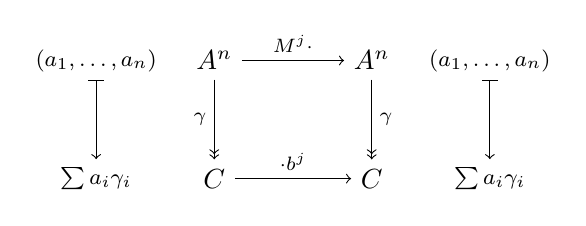
\begin{tikzpicture}
 	\node (a) at (0,1.5) {$A^n$};
 	\node (b) at (2,1.5) {$A^n$};
 	\node (c) at (0,0) {$C$};
 	\node (d) at (2,0) {$C$};
 	\begin{scriptsize}
	 	\draw[->] (a) -- (b) node[pos=0.5,above] {$M^j\cdot$};
	 	\draw[->>] (a) -- (c) node[pos=0.5, left] {$\gamma$};
	 	\draw[->>] (b) -- (d) node[pos=0.5,right] {$\gamma$};
	 	\draw[->] (c) -- (d) node[pos=0.5, above] {$\cdot b^j$};
 	\end{scriptsize}
 	\begin{footnotesize}
	 	\node (a1) at (-1.5,1.5) {$(a_1,\ldots,a_n)$};
	 	\node (c1) at (-1.5,0) {$\sum a_i\gamma_i$};
	 	\draw[|->] (a1) -- (c1);
	 	\node (b1) at (3.5,1.5) {$(a_1,\ldots,a_n)$};
	 	\node (d1) at (3.5,0) {$\sum a_i\gamma_i$};
	 	\draw[|->] (b1) -- (d1);
 	\end{footnotesize}
 	\end{tikzpicture}
  \end{center}
  commutes) it follows, that $b^n \cdot c = \sum_{i=0}^{n-1} p_ib^ic$ (first for $c=\gamma_i$, then all of $C$). Taking $c=1$ shows $b^n = \sum_{i=0}^{n-1}p_i b^i$ as stated.
  \item If $C$ is as in $A$ and contains $b_1, b_2$, then it contains $b_1\pm b_2$ and $b_1\cdot b_2$, showing that these are integral over $A$. 
  \item Let, more generally, $B/A$ be integral and $c\in C$ integral over $B$. It satisfies an equation $c^d = \sum_{i=0}^{d-1} \beta_i c^i$ with $\beta_i\in B$. By a), there is an $A$-subalgebra $\tilde B\subseteq B$ which is finite over $A$ and contains the $\beta_i$. Then $c$ is integral over $\tilde B$, hence by a) there is a $\tilde B$-subalgebra $\tilde C\subseteq C$ containing $c$ and finite over $\tilde B$. Now $\tilde C/A$ is finite by Proposition \ref{prop:1.4.1}b), hence $c$ is integral over $A$ by a).
  %end 2017-04-27
%start 2017-05-4
\item Suppose that $B$ is a field and let $a\in A \setminus\{0\}$. Since $B/A$ is integral, we can find $\alpha_0\ldotspam \alpha_{n-1}\in A$ such that 
\begin{align*}
 \left(a^{-1}\right)^n+\sum_{i=0}^{n-1}\alpha_i\cdot\left(a^{-1}\right)^i = 0.
\end{align*}
But then 
\begin{align*}
 a^{-1} = a^{n-1}\left(a^{-1}\right)^n = -\sum_{i=0}^{n-1} \alpha_i\cdot a^{n-1} \in A.
 \end{align*}
So every element of $A\setminus\{0\}$ is an unit and $A$ a field.
 \end{alphanumerate}
\end{proof}
\begin{rem}
 Cayley-Hamilton (similar to other determinant identities) can be derived from the case of algebraically closed fields by embedding integer domains into the algebraic closures of their quotient fields. Fir arbitrary rings $R$ (possibly with zero divisors) one may consider the surjective ring homomorphism
 \begin{align*}
  \Z[X_r: r\in R] &\longto R\\
  X_r &\longmapsto r
 \end{align*}
 and then reduce to the case of integer domains which was done above.

\end{rem}
\begin{cor}
 A ring extension is finite iff it is integral and of finite type.
\end{cor}
\begin{rem}
 Algebraic independence over $k$ means that
 \begin{align*}
  \sum_{\alpha\in \N^n} \lambda_{\alpha_1\ldotspam \alpha_n} a_1^{\alpha_1}\cdot\ldots\cdot a_n^{\alpha_n}=0
 \end{align*}
implies that each $\lambda_{\alpha_1\ldotspam \alpha_n}=0$. Equivalently, the ring homomorphism 
\begin{align*}
 k[X_1,\ldots, X_n]&\longto k[a_1,\ldots, a_n]\\
 X_i&\longmapsto a_i
\end{align*}
is injective, hence $k[X_1,\ldots, X_n]\simeq k[a_1,\ldots, a_n]$ as $k$-algebras.
\end{rem}

\begin{thm}\label{thm:NoetherNormalization}
 Let $k$ be a field, $A$ a $k$-algebra of finite type over $k$. Then there are over $k$ algebraically independent $a_1\ldotspam a_n\in A$ such that $A/k[a_1\ldotspam a_n]$ is integral.
\end{thm}
\begin{proof}
 Since $A$ is of finite type over $k$, we can choose $a_1,\ldots, a_n$ such that $A$ is integral over $k[a_1,\ldots, a_n]$ (e.g. choose the $a_i$ as generators of $A$ as $k$-algebra). We may choose a minimal $n$ such that this is possible. We claim 
 \begin{description}
  \item [$\ast$] Let $x_1,\ldots, x_n\in A$ such that $A$ is integral over $k[x_1,\ldots,x_n]$ and $n$ is minimal having this property that such $x_i$ exist. Then the $x_i$ are algebraically independent over $k$.
 \end{description}
Write $x^\alpha = \prod_{i=1}^n x_i^{\alpha_i}$ for short. Suppose that
\begin{align*}
\sum_{\alpha\in\N_0^n} \lambda_\alpha \cdot x^\alpha =0\label{eq:1.5.1a}\tag{\#}
\end{align*}
where 
\begin{align*}
 S\coloneqq \left\{\alpha\in\N_0^n\middle| \lambda_\alpha\neq 0\right\}
\end{align*}
 is finite but not empty. Let $y_1=x_1$ and $y_k = x_k +y_1^{d_k}$ (the $d_i$ will be chosen later on). Since the $x_i$ can be recovered from the $y_i$, we have $k[x_1,\ldots,x_n] = k[y_1,\ldots,y_n]$. The idea is to choose the $d_i$ such that $y_1$ is integral over $k[y_2,\ldots,y_n]$. Then $A$ is integral over $k[y_2,\ldots,y_n]$, contradicting the minimality of $n$. 

Let $\omega_d(\alpha) =\alpha_1 +\sum_{i=2}^nd_i\cdot \alpha_i$. The summands can be expressed as 
\begin{align*}
 \lambda_\alpha x^\alpha &= \lambda_\alpha y_1^{\alpha_1} \cdot\prod_{i=2}^n \left(y_i - y_1^{d_i}\right)^{\alpha_i} \\
 &= \pm \lambda_\alpha y_1^{\omega_d(\alpha)} + \sum_{j=0}^{\omega_d(\alpha)-1} Q_{\alpha,j}(y_2,\ldots, y_n) y_1^j
\end{align*}
if all $d_k$ are positive. Here $Q_{\alpha, j}$ denotes some polynomial. 

If $d_2,\ldots, d_n$ can be chosen in such a way that
\begin{align*}
 \omega_d: S\longto \N
\end{align*}
has a unique maximum $\alpha^\ast \in S$, the relation \ref{eq:1.5.1a} becomes
\begin{align*}
 0 = \lambda_{\alpha^\ast} y_1^{\omega_d(\alpha^\ast)} +\sum_{j=0}^{\omega_d(\alpha^\ast)-1} Q_j(y_2,\ldots,y_n)y_1^j
\end{align*}
proving, that $y_1$ is integral over $k[y_2,\ldots,y_n]$. 

Now $d_2,\ldots,d_n$ can be chosen in several ways. For example, take
\begin{align*}
 A = \max\left\{l\in\N: \text{ there is }\alpha\in S \text{ such that } l =\alpha_i \text{ for some } i\right\}
\end{align*}
and chose $d_i = (A+1)^{i-1}$. Then $\omega_d$ is injective since the $(A+1)-$adic representation of an integer is unique.
 \end{proof}


\subsection{Proof of the Nullstellensatz and some consequences}\label{sec:ProofNullstellensatz}
\begin{thm}\label{thm:fieldExtensionOfFiniteTypeIsFinite}
 Let $L/K$ be a field extension such that $L$ is a $K$-algebra of finite type. Then $L/K$ is finite.
\end{thm}
\begin{proof}
By Noether's Normalization Theorem (Theorem \ref{thm:NoetherNormalization})  there are $y_1, \ldots, y_n\in L$ algebraically independent over $K$ such that $L$ is integral over $K[y_1,\ldots,y_n]$. By Proposition \ref{prop:integralStuff} d), $K[y_1,\ldots,y_n]$ is a field. But as $y_1,\ldots, y_n$ are algebraically independent, $K[y_1,\ldots, y_n]$ is isomorphic to the polynomial ring $K[X_1,\ldots,X_n]$, which is only a field for $n=0$. Thus $L/K$ is integral (i.e. algebraic) and since the extension is finitely generated it must be finite. 
\end{proof}
\begin{rem}
 When $K$ is uncountable and $\lambda\in L$ non-algebraic over $K$, the subfield $K(\lambda)$ is isomorphic to $K(X)$, the field of rational functions over $K$, which has uncountable dimension as a $K$-vector space as the $\frac{1}{X-\gamma}$, $\gamma\in K$, are linearly independent. But the dimension (as a $K$-vector space) of a $K$-algebra must be countable, as there are only countable many monomials in finitely many elements.
\end{rem}
\begin{cor}
 Let $k$ be a field, $\mathfrak{m}\subseteq k[X_1,\ldots,X_n]$ a maximal ideal, then it's residue field $k[X_1,\ldots,X_n]/\mathfrak{m}$ is a finite field extension of $k$.
\end{cor}
\begin{proof}
 Indeed, it is generated by $X_1+\mathfrak{m},\ldots, X_n+\mathfrak{m}$ and thus finite over $k$.
\end{proof}






\end{document}
